\subsection{Measurements in the Past}

ATGC parameters of $WW\gamma$ vertex can be probed in $W\gamma$, $WW$, and $WZ$ measurements. Limits on $\Delta \kappa_\gamma$ and $\lambda_\gamma$ constants from different D0 \cite{ref_D0_aTGC_comb}, LEP \cite{ref_LEP_aTGC_comb}, ATLAS \cite{ref_7TeV_ATLAS}, \cite{ref_ATLAS_WW_8TeV}, \cite{ref_ATLAS_VW_8TeV} and CMS \cite{ref_7TeV_CMS}, \cite{ref_CMS_WW_7TeV}, \cite{ref_CMS_WW_8TeV}, \cite{ref_CMS_VW_7TeV} measurements are summarized in Fig.~\ref{fig:aTGC_cg}.\\ 

\begin{figure}[htb]
  \begin{center}
    {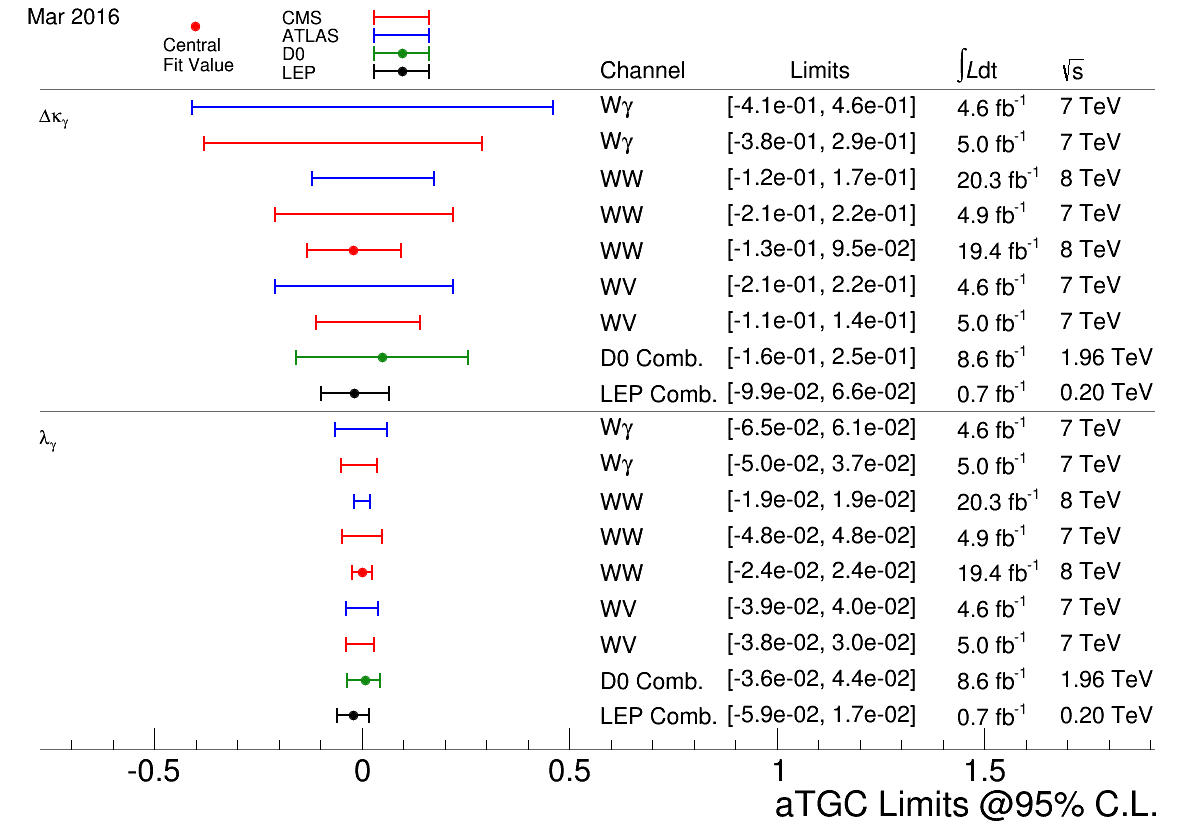
\includegraphics[width=0.80\textwidth]{../figs/WgAbout/aTGC_cg.png}}
    \caption{Summary of limits on the $WW\gamma$ aTGC coupling constants. Figure from \cite{ref_twiki_SMP_ATGC}}
    \label{fig:aTGC_cg}
  \end{center}
\end{figure}

The most recent measurements of $W\gamma$ production were performed by CMS \cite{ref_7TeV_CMS} and ATLAS \cite{ref_7TeV_ATLAS} collaborations with $pp$ collisions at $\sqrt{s}=7$~GeV collected in 2011. The measurements are based on~5~fb$^-1$ and~4.6~fb$^-1$ of integrated luminosity with CMS and ATLAS respectively. Both collaborations considered two channels: $W\gamma\rightarrow\mu\nu\gamma$ and $W\gamma\rightarrow e\nu\gamma$.\\

%Introduce variables
To determine a kinematics of a particle in CMS or ATLAS, three variables are used: a transverse momentum component $P_T$, an azimuthal angle in the $r-\phi$ plane of a detector (perpendicular to the beam direction) $\phi$ and a pseudorapidity $\eta=-\ln[\tan(\theta/2)]$. For photon sometimes notation $E_T^\gamma$ (transverse energy) is used instead of $P_T^\gamma$. Since photon is massless, transverse energy of a photon equals to its transverse momentum.\\

Defining a kinematics of a potential neutrino, we use a missing transverse energy $MET$ and corresponding to it azimuthal angle $\phi$. Missing longitudial component is not reconstructed because total longitudial momentum of initial state quarks in a $pp$ collision is not known, and, therefore, it is not possible to compute how much of the longitudial momentum is missing.\\  

The process signature of $W\gamma$ is a prompt, isolated photon, a prompt isolated energetic lepton ($\mu$ or e) and a significant missing trensverse energy due to the neutrino. \\

%Trigger\\
In CMS measurement, for the $W\gamma\rightarrow\mu\nu\gamma$ events the isolated single muon trigger was used, it includes requirements of $p_T^{\mu}>$30 GeV and $|\eta^{\mu}|<$2.4(2.1) for Run 2011A(2011B). For the electron channel, the isolated single electron trigger was used. The trigger requirements were $p_T^e>$32 GeV except a small fraction of data where it was $p_T^e>$27 GeV, $|\eta_3|>$3, $M_T^W>$50 GeV, where $M_T^W=\sqrt{2 \cdot p_T^e \cdot MET \cdot (1-cos\Delta\phi(e,MET))}$ is a transverse mass of a $W$ boson.\\

In the ATLAS measurement, the single electron, single muon and single photon triggers were used with $P_T$ thresholds of $P_T^e>20(22)$~GeV depending on a run range, $P_T^\mu>18$~GeV, $P_T^\gamma>80$~GeV.\\

%Event selection\\
The event-level selection requirements in CMS included one well-identified lepton with kinematic requirements $p_T^l>$35~GeV, $|\eta^\mu|<$2.1, $\eta^e<$2.5, one well-identified photon with $p_T^\gamma>15$~GeV, $|\eta^\gamma|<$2.5, and $M_W^T>$70~GeV. To reject events from $Z\gamma\rightarrow ll\gamma$ process, events with the second reconstructed lepton of the same flavor were vetoed. The second muon veto requirements included $p_T^\mu>$10~GeV, $|\eta^\mu|<$2.4. The second electron veto requirements included $p_T^\mu>$20~GeV, $|\eta^\mu|<$2.5, and weak electron identification criteria. The separation between a photon and a lepton were required to be $\Delta R(l,\gamma) = \sqrt{\Delta \eta(l,\gamma)^2 + \Delta \phi(l,\gamma)^2}>$0.7.\\  

ATLAS collaboration also required each candidate event to have an exactly one lepton, at least one isolated photon and a significant missing transverse energy. The phase space requirements are the same as those for CMS: $p_T^{\gamma}>15$~GeV and $\Delta R(l,\gamma)>$0.7 however other selection critea are slightly different: $p_T^l>25$~GeV, $E_T^{miss}>35$~GeV, $M_T^W>40$~GeV. In the electron channel Z mass window cut was applied to reduce the contribution from $Z\rightarrow e^+e^-$ events.\\

%CMS PHASE SPACE:\\

%The phase space requirements in CMS were $p_T^\gamma>15$~GeV and  $\Delta R(l,\gamma)>$0.7. Requirements on $P_T^\gamma$ and $\Delta R$ are necessary to avoid the divergence of the total cross section and also to supress the contribution from the FSR diagram and, therefore, make the TGC contribution more significant.\\

%Muon\\

%Electron\\

%Photon\\

%MET\\

%Background Estimation\\

%Events selected according with the described criteria represent a mixture of the signal and background events. The major source of the background is the fake photon background where hadronic jets are misidentified as photons. Such events originate from $W+$jets process mostly but $Z+$jets and $\bar{t}t+$jets events contribute to this source of the background as well. The template method was used as a major method to estimate this background. The shower-shape variable $\sigma_{i\eta i\eta}^{\gamma}$ was used as a discrimination variable. The ratio method was used as a cross check by measuring and comparing the probabilities for jets to pass photon or jets selection criteria. \\

%Other sources of backgrounds include real-$\gamma$ backgrounds, fake lepton + real photon and fake lepton + fake photon sources.\\ 

The $p_T^\gamma$ spectra of the selected events in data superimposed with selected events in the simulation of the signal and estimated background contribution for the muon and electron channels are shown in Fig.~\ref{fig:Wg7TeV_CMS_ptGamma} for CMS and in Fig.~\ref{fig:Wg7TeV_ATLAS_ptGamma} for ATLAS. \\

The major source of the background is the fake photon background where hadronic jets are misidentified as photons. Such events originate from $W+$jets process mostly but $Z+$jets and $\bar{t}t+$jets events contribute to this source of the background as well. The second major background for the electron channel is the fake photon background where electron can be misidentified as a photon.  Such events are coming from $Z+$jets events. Other sources of backgrounds include real-$\gamma$ backgrounds, fake lepton + real photon and fake lepton + fake photon sources. Fig.~\ref{fig:Wg7TeV_CMS_ptGamma} and Fig.~\ref{fig:Wg7TeV_ATLAS_ptGamma} show a good agreement.\\

%Diboson processes contribute to this background for both channels. The fake rates are estimated from the $Z\rightarrow ee$ sample, by checking how often one of the electrons would pass photon selection criteria given the other one passed stringent electron selection criteria.The figure shows a good agreement within the estimated uncertainties. \\

\begin{figure}[htb]
  \begin{center}
    {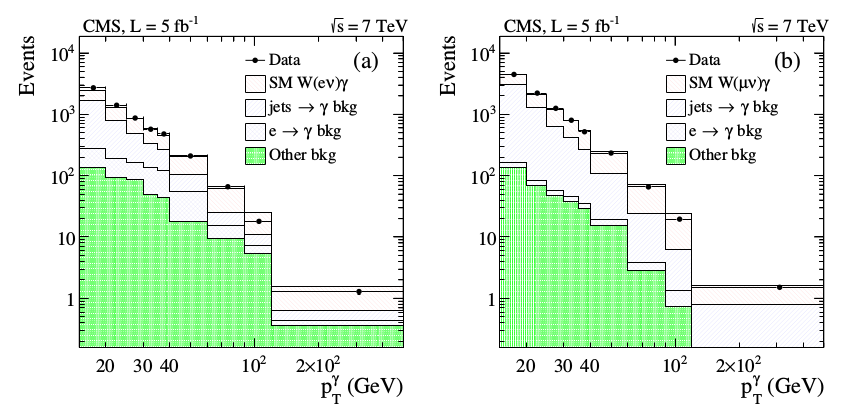
\includegraphics[width=0.80\textwidth]{../figs/WgAbout/Wg7TeV_CMS_ptGamma.png}}
    \caption{The distribution fo the $p_T^\gamma$ of W$\gamma$ candidates in the analysis of 7 TeV CMS data. Data vs signal MC + background estimates. Left: $W\gamma\rightarrow e\nu\gamma$, right: $W\gamma\rightarrow \mu\nu\gamma$ \cite{ref_7TeV_CMS}.}
    \label{fig:Wg7TeV_CMS_ptGamma}
  \end{center}
\end{figure}

\begin{figure}[htb]
  \begin{center}
    {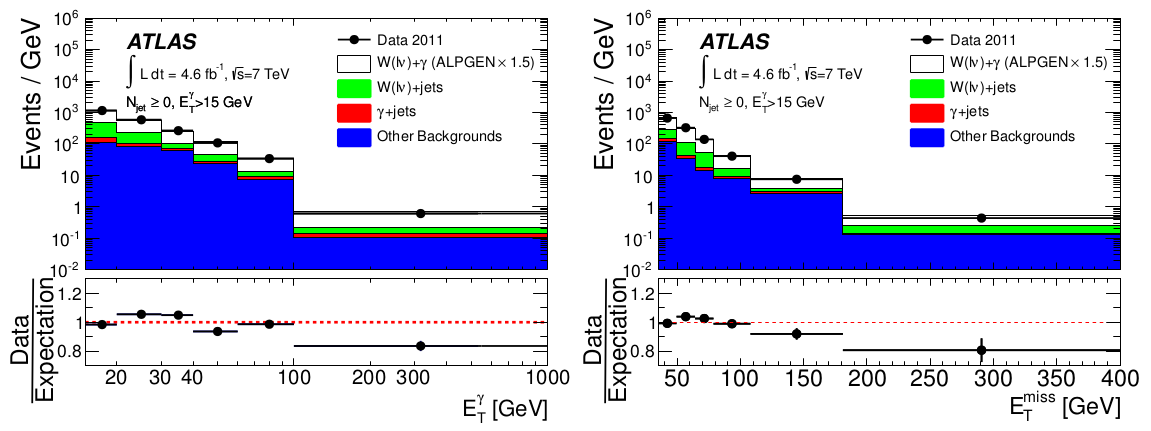
\includegraphics[width=0.80\textwidth]{../figs/WgAbout/Wg7TeV_ATLAS_ptGamma.png}}
    \caption{The distribution fo the $p_T^\gamma$ (left) and $E_T^\gamma$ (right) of W$\gamma$ candidates in the analysis of 7 TeV ATLAS data. Data vs signal MC + background estimates \cite{ref_7TeV_ATLAS}. }
    \label{fig:Wg7TeV_ATLAS_ptGamma}
  \end{center}
\end{figure}

CMS provides measurements of the $P_T^\gamma$ spectrum, the total cross section within the phase spaces of $\Delta R>0.7$, $P_T^\gamma>15$~GeV, $P_T^\gamma>60$~GeV and $P_T^\gamma>90$~GeV, and limits on aTGC coupling constants.\\

ATLAS, in addition to the $P_T^\gamma$ spectrum, total cross section and limits, provides the differential cross section and cross section with different number of associated jets. No evidence of a new physics is observed.\\

%The estimated cross sections are:\\
%$\sigma(pp\rightarrow W\gamma \rightarrow e\nu\gamma)$=36.6$\pm$1.2(stat.)$\pm$4.3(syst.)$\pm$0.8(lumi) pb\\
%$\sigma(pp\rightarrow W\gamma \rightarrow \mu\nu\gamma)$=37.5$\pm$0.9(stat.)$\pm$4.4(syst.)$\pm$0.8(lumi) pb\\
%And the combination result:\\
%$\sigma(pp\rightarrow W\gamma \rightarrow l\nu\gamma)$=37.0$\pm$0.8(stat.)$\pm$4.0(syst.)$\pm$0.8(lumi) pb\\

%The paper also provides the cross section measurements for $p_T^\gamma>$60 GeV and for $p_T^\gamma>$90 GeV. The combination of two channels for $p_T^\gamma>$60 GeV is $\sigma=$0.76$\pm$0.05(stat.)$\pm$0.08(syst.)$\pm$0.02(lumi) pb while the theoretical NLO prediction is $\sigma=$0.58$\pm$0.08 pb. The result for $p_T^\gamma>$60 GeV is $\sigma=$0.200$\pm$0.025(stat.)$\pm$0.038(syst.)$\pm$0.004(lumi) pb while the theoretical NLO prediction is $\sigma=$0.173$\pm$0.026 pb.\\

% ADD CONCLUSIONS

%Background Estimation
%AccXEff
%Pt Spectrum
%Differential and Total CS

%Wg 8 TeV at ATLAS (?)
%NO. DOES NOT EXIST
